%% Dexter Barrows, 2016
%% dbarrows.github.io

\section{S-maps}

    A family of forecasting methods that shy away from the mechanistic model-based approaches outlined in the previous sections have been developed by Sugihara (references) over the last several decades. As these methods do not include a mechanistic model in their forecasting process, they also do not attempt to perform parameter estimation or inference. Instead they attempt to reconstruct the underlying dynamical process as a weighted linear model from a time series.

    One such method, the sequential locally weighted global linear maps (S-map), builds a global linear map model and uses it to produce forecasts directly. Despite relying on a linear mapping, the S-map does not assume the time series on which it is operating is the product of linear system dynamics, and in fact was developed to accommodate non-linear dynamics. The linear component of the method only comes into play when combining forecast components together to produce a single estimate

    The S-map works by first constructing a time series embedding of length $E$, known as the library and denoted $\{\mathbf{x_i}\}$. Consider a time series of length $T$ denoted $x_1, x_2,..., x_T$. Each element in the time series with indices in the range $E,E+1,...,T$ will have a corresponding entry in the library such that a given element $x_t$ will correspond to a library vector of the form $\mathbf{x_i} = (x_t, x_{t-1},...,x_{t-E+1})$. Next, given a forecast length $L$ (representing $L$ time steps into the future), each library vector $\mathbf{x_i}$ is assigned a prediction from the time series $y_i = x_{t+L}$, where $x_t$ is the first entry in $\mathbf{x_i}$. Finally, a forecast ${\hat{y_t}}$ for specified predictor vector $\mathbf{x_t}$ (usually from the library itself), is generated using an exponentially weighted function of the library $\{\mathbf{x_i}\}$, predictions $\{y_i\}$, and predictor vector $\mathbf{x_t}$.

    This function is defined as follows:

    First construct a matrix $A$ and vector $b$ defined as

    \begin{equation}\label{AB}
    	\begin{array}{rl}
        \displaystyle
            A(i, j) & = w (||\mathbf{x_i}-\mathbf{x_t}||) \mathbf{x_i}(j) \\
            b(i) 	& = w (||\mathbf{x_i}-\mathbf{x_t}||) y_i
        \end{array}
    \end{equation}

    where $||\cdot||$ is the Euclidean norm, $i$ ranges over 1 to the length of the library, and $j$ ranges over $[0,E]$. In the above equations and the ones that follow, we set $x_t(0) \equiv 1$ to account for the linear term in the map.

	The weighting function $w$ is defined as

	\begin{equation}
		w(d) = \exp \left( \frac{-\theta d}{\bar{d}} \right) ,
	\end{equation}

	where $d$ is the euclidean distance between the predictor vector and library vectors in Equation [\ref{AB}] and $\bar{d}$ is the average of these distances. We can then see that $\theta$ serves as a way to specify the appropriate level of penalization applied to poorly-matching library vectors -- if $\theta$ is 0 all weights are the same (no penalization), and increasing $\theta$ increases the level of penalization.

	Now we solve the system $Ac = b$ to obtain the linear weightings used to generate the forecast according to

	\begin{equation}
		\hat{y_t} = \sum_{j = 0}^{E} c_t(j) \mathbf{x_t}(j) .
	\end{equation}

	In this way we have produced a forecast value for a single time. This process can be repeated for a sequence of times $T + 1, T + 2, ...$ to project a time series into the future.

	In essence what we are doing is generating a series of forecasts from every vector in the library, weighting those forecasts based on how similar the corresponding library vector is to our predictor vector, obtaining a solution to the system that maps components of a predictor vector to its library vector's forecasted point (the mapping), then applying that mapping to our predictor variable to obtain a forecast.


\section{S-map Algorithm}

    The above description can be summarized in Algorithm [\ref{smap}].

    \begin{algorithm}

        \BlankLine

        \SetKwInOut{Input}{Input}
        \SetKwInOut{Output}{Output}
        \DontPrintSemicolon

        \tcc{Select a starting point}
        \Input{Time series $x_1, x_2, ..., x_T$, embedding dimension $E$, distance penalization $\theta$, forecast length $L$, predictor vector $\mathbf{x_t}$}

        \BlankLine

        \tcc{Construct library $\{{\mathbf{x_i}}\}$}
        \For{$i = E:T$}{
        	$\mathbf{x_i} = (x_i, x_{i-1}, ...,x_{i-E-1})$
        }

        \BlankLine

        \tcc{Construct mapping from library vectors to predictions}
        \For{$i = 1:(T_E+1)$}{
        	\For{$j = 1:E$}{
	        	$A(i,j) = w(||\mathbf{x_i} - \mathbf{x_t}||) \mathbf{x_i}(j)$
	        }
        }
        \For{$i = 1:(T_E+1)$}{
	        $b(i) = w(||\mathbf{x_i} - \mathbf{x_t}||) y_i$
        }

        \BlankLine

        \tcc{Use SVD to solve the mapping system, Ac = b}
        $SVD(Ac = b)$

        \BlankLine

        \tcc{Compute forecast}
        $\hat{y_t} = \sum_{j = 0}^{E} c_t (j) \mathbf{x_t} (j)$

        \BlankLine

        \tcc{Forecasted value in time series}
        \Output{Forecast $\hat{y_t}$}

        \BlankLine

        \caption{S-map \label{smap}}

    \end{algorithm}


\section{SIRS Model}

	In an epidemic or infectious disease context, the S-map algorithm will only really work on time series that appear cyclic. While there is nothing mechanically that prevents it from operating on a time series that do not appear cyclic, S-mapping requires a long time series in order to build a quality library. Without one the forecasting process would produce unreliable data.

	Given, the S-map's data requrements, we need to specify a modified version of the SIR model. As IF2 and HMCMC in principle should be able operate on any reasonably well-specified model, the easiest way to compare the efficacy of S-mapping to IF2 or HMCMC is to generate data from a SIRS model with a seasonal component, and have all methods operate on the resulting time series.

	The basic skeleton of the SIRS model is similar to the stochastic SIR model described previously, with one small addition. The deterministic ODE component of the model is as follows.

	\begin{equation}
		\begin{aligned}
			\frac{dS}{dt} & = - \Gamma(t) \beta S I + \eta R \\
			\frac{dI}{dt} & = \Gamma(t) \beta S I - \gamma I \\
			\frac{dR}{dt} & = \gamma I - \eta R,
		\end{aligned}
	\end{equation}

	There are two new features here. We have a rate or waning immunity $\eta$ through which people become able to be reinfected, and a seasonality factor function $\Gamma (t)$ defined as

	\begin{equation}
		\Gamma(t) = \exp \left[ 2 \left( \cos \left(  \frac{2 \pi}{365} t \right) - 1 \right) \right].
	\end{equation}

	This function oscillates between 1 and $e^{-4}$ (close to 0) and is meant to represent transmission damping during the off-season, for example summer for influenza. Further, it displays flatter troughs and sharper peaks to exaggerate its effect in peak season.

	As before, $\beta$ is allowed to walk restricted by a geometric mean, described by

	\begin{equation}
		\beta_{t+1} = \exp \left( \log(\beta_{t}) + \eta (\log(\bar{\beta}) - \log(\beta_{t})) + \epsilon_{t} \right).
	\end{equation}

	Figure [\ref{sirsdataplot}] shows the SIRS model simulated for the equivalent of 5 years (260 weeks) and adding noise drawn from $\mathcal{N}(0,\sigma)$.

	\begin{figure}
        \centering
        \captionsetup{width=.8\linewidth}
        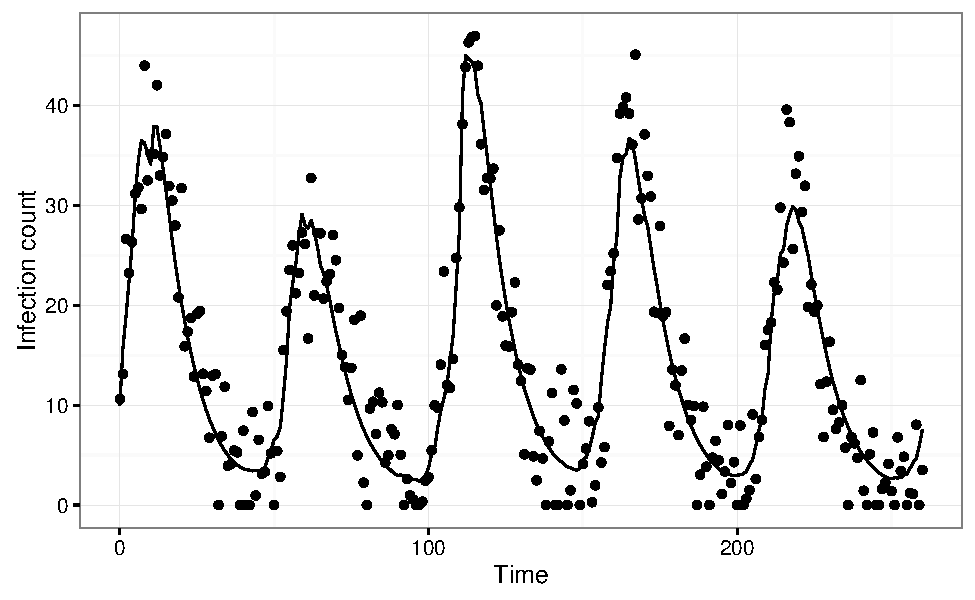
\includegraphics[width=0.8\textwidth]{./images/dataplot.pdf}
        \caption{Five cycles generated by the SIRS function. The solid line the the true number of cases, dots show case counts with added observation noise. The parameter values were $R_0 = 3.0$, $\gamma = 0.1$, $\eta = 1$, $\sigma = 5$, and 10 initial cases. \label{sirsdataplot}}
    \end{figure}

    Figure [\ref{smap_project}] shows how the S-map can reconstruct the next cycle in the time series.

    \begin{figure}[H]
        \centering
        \captionsetup{width=.8\linewidth}
        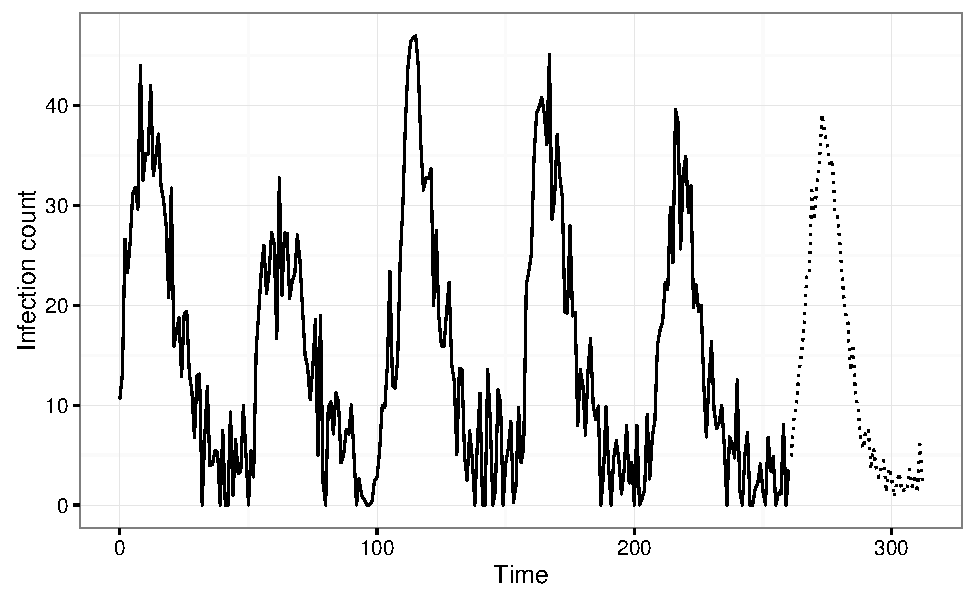
\includegraphics[width=0.8\textwidth]{./images/smap-project.pdf}
        \caption{S-map applied to the data from the previous figure. The solid line shows the infection counts with observation noise from the previous plot, and the dotted line is the S-map forecast. Parameters chosen were $E = 14$ and $\theta = 3$. \label{smap_project}}
    \end{figure}

    The parameters used in the S-map algorithm to obtain the forecast used in Figure [\ref{smap_project}] were obtained using a grid search of potential parameters outlined in [\textit{Sugihara ref}]. The script to perform this optimisation procedure is included in the appendices.


\section{SIRS Model Forecasting}

	Naturally we wish to compare the efficacy of this comparatively simple technique against the more complex and more computationally taxing frameworks we have established to perform forecasting using IF2 and HMCMC.

	To do this we generated a series of artificial time series of length $260$ meant to represent 5 years of weekly incidence counts and used each method to forecast up to 2 years into the future. Our goal here was to determine how forecast error changed with forecast length.

	Figure [\ref{sirssseplot}] shows the results of the simulation.

	\begin{figure}
        \centering
        \captionsetup{width=.8\linewidth}
        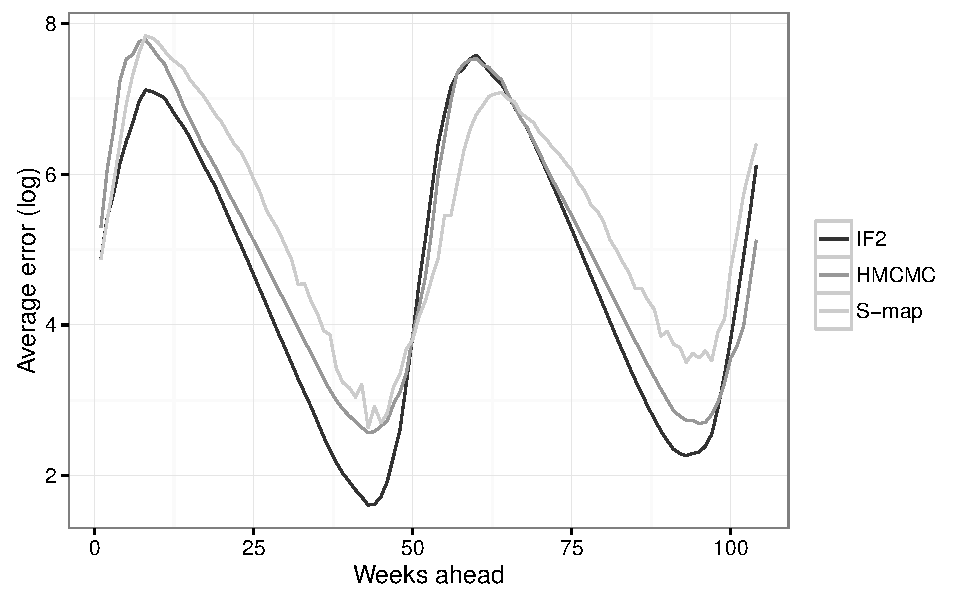
\includegraphics[width=0.8\textwidth]{./images/sseplot.pdf}
        \caption{Error as a function of forecast length. \label{sirssseplot}}
    \end{figure}

    Interestingly, all methods produce roughly the same result, which is to say the spikes in each outbreak cycle are difficult to accurately predict. IF2 produces better results than either HMCMC and the S-map for the majority of forecast lengths, with the S-map producing the poorest results with the exception of the second rise in infection rates where it outperforms the other methods.

    While the S-map may not provide the same fidelity or forecast as IF2 or HMCMC, it shines when it comes to running time. Figure [\ref{sirstimeplot}] shows the running times over 20 simulations.

    \begin{figure}
        \centering
        \captionsetup{width=.8\linewidth}
        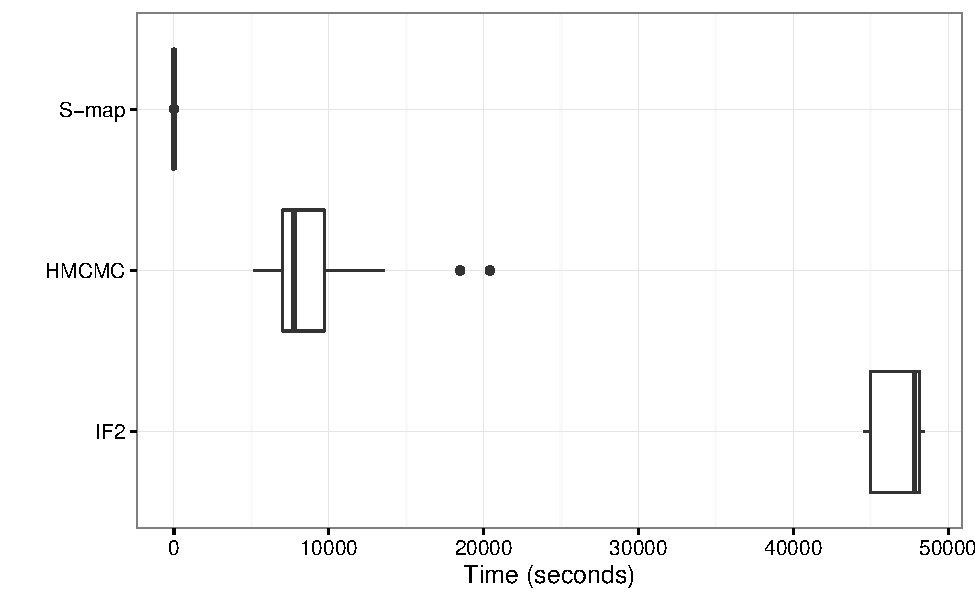
\includegraphics[width=0.8\textwidth]{./images/timeplot.pdf}
        \caption{Runtimes for producing SIRS forecasts. The box shows the middle 50th quantile, the bold line is the median, and the dots are outliers. Note that these are not ``true'' outliers, simply ones outside a ranges based on the interquartile range. \label{sirstimeplot}}
    \end{figure}

    It is clear from Figure [\ref{timeplot}] that the S-map running times are minute compared to the other methods, but to emphasize the degree: The average running time for the S-map is about $0.15$ seconds, for IF2 it is about $47,000$, and for HMCMC it is about $9,200$. This is a speed-up of over 316,000x compared to IF2 and over 61,800x compared to HMCMC.
